% sections/05_robustness.tex
\section{Robustness Check}
\label{sec:robustness}

The previous two sections showed that adding sex to the predictors improves species classification with logistic regression and body mass regression with both models. Those improvements could be a real effect of sex, or they could be an artifact of the particular rows that ended up in the training set. To distinguish the two cases, the training data is split into two disjoint halves and each model is trained twice, once on each half, always evaluated against the same test set.

\subsection{Design of the A/B Split}

The master train/test split is performed once, by row index, on the preprocessed frame. The test set is 20 \% of the rows and is stratified by species. The remaining 80 \% is partitioned into two disjoint halves of equal size, \texttt{train\_A} and \texttt{train\_B}, using a different random seed. The two halves are disjoint and their union equals the full training set. All feature configurations, all models and both studies use this same partition, so any difference between \texttt{train\_A} and \texttt{train\_B} comes from the training sample, not from a different test set or a different preprocessing step.

\subsection{Stability in Classification}

Table~\ref{tab:cls_stability} reports the accuracy of each classifier on the shared test set, for the two feature configurations and the two training subsets.

\begin{table}[htbp]
	\centering
	\caption{Classification accuracy across training subsets. The delta column is the change in accuracy when sex is added.}
	\label{tab:cls_stability}
	\begin{tabular}{llccc}
		\toprule
		Model & Subset & Without sex & With sex & Delta \\
		\midrule
		Logistic regression & train\_A & 0.925 & 0.970 & +0.045 \\
		Logistic regression & train\_B & 0.925 & 0.985 & +0.060 \\
		Decision tree       & train\_A & 0.910 & 0.910 & 0.000 \\
		Decision tree       & train\_B & 0.955 & 0.955 & 0.000 \\
		\bottomrule
	\end{tabular}
\end{table}

For logistic regression the delta is positive in both subsets, with a range of 0.045 to 0.060. The sign is the same in both runs, so the effect is stable with respect to the training sample. The magnitude varies, which is expected given that the test set has 67 rows and the standard error of an accuracy estimate at that size is close to 0.03. For the decision tree the delta is exactly zero in both subsets. The tree is not unstable, it is simply indifferent to sex: the splits it chooses already encode the information that sex provides.

\begin{figure}[htbp]
	\centering
	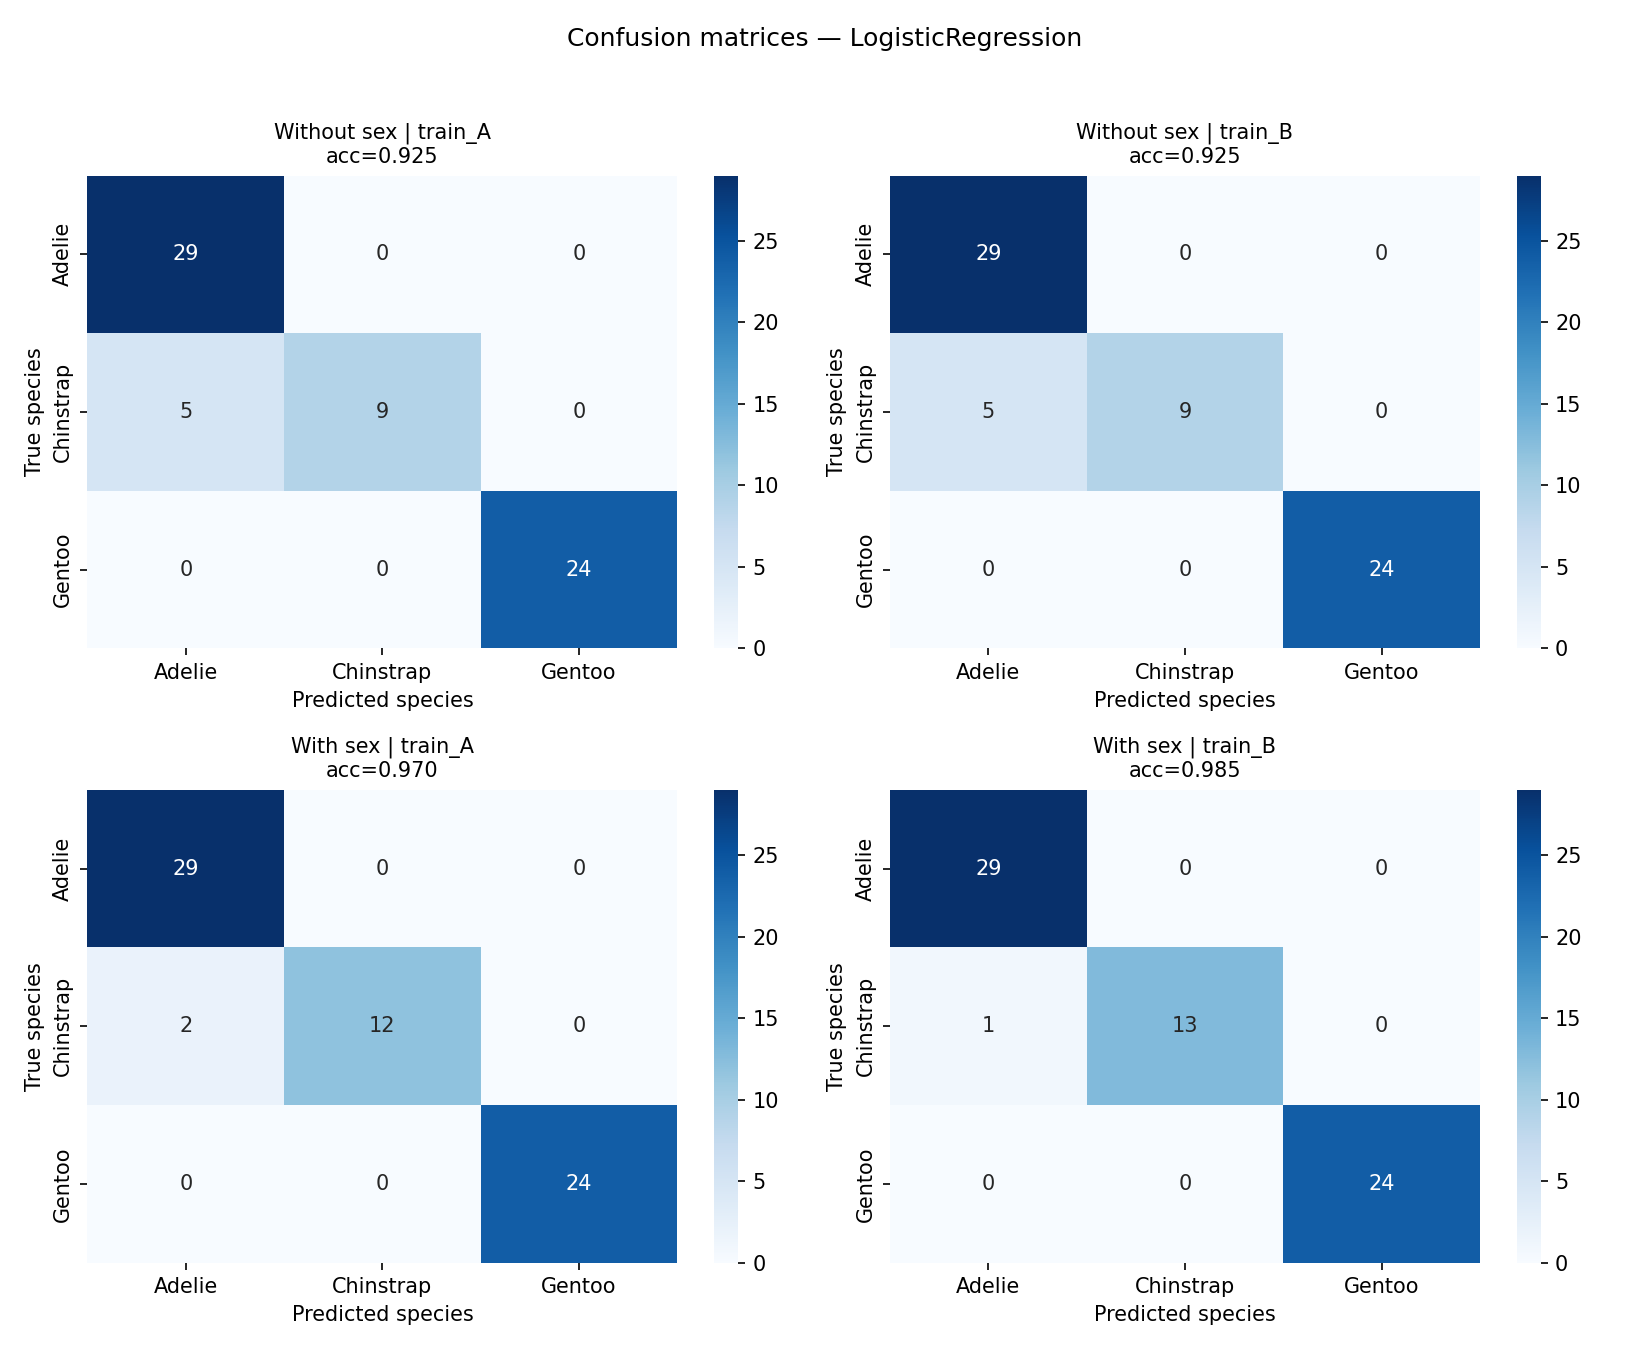
\includegraphics[width=0.95\textwidth]{figures/grid_LogisticRegression.png}
	\caption{Confusion matrices for logistic regression across feature configurations and training subsets.}
	\label{fig:grid_logreg}
\end{figure}

\begin{figure}[htbp]
	\centering
	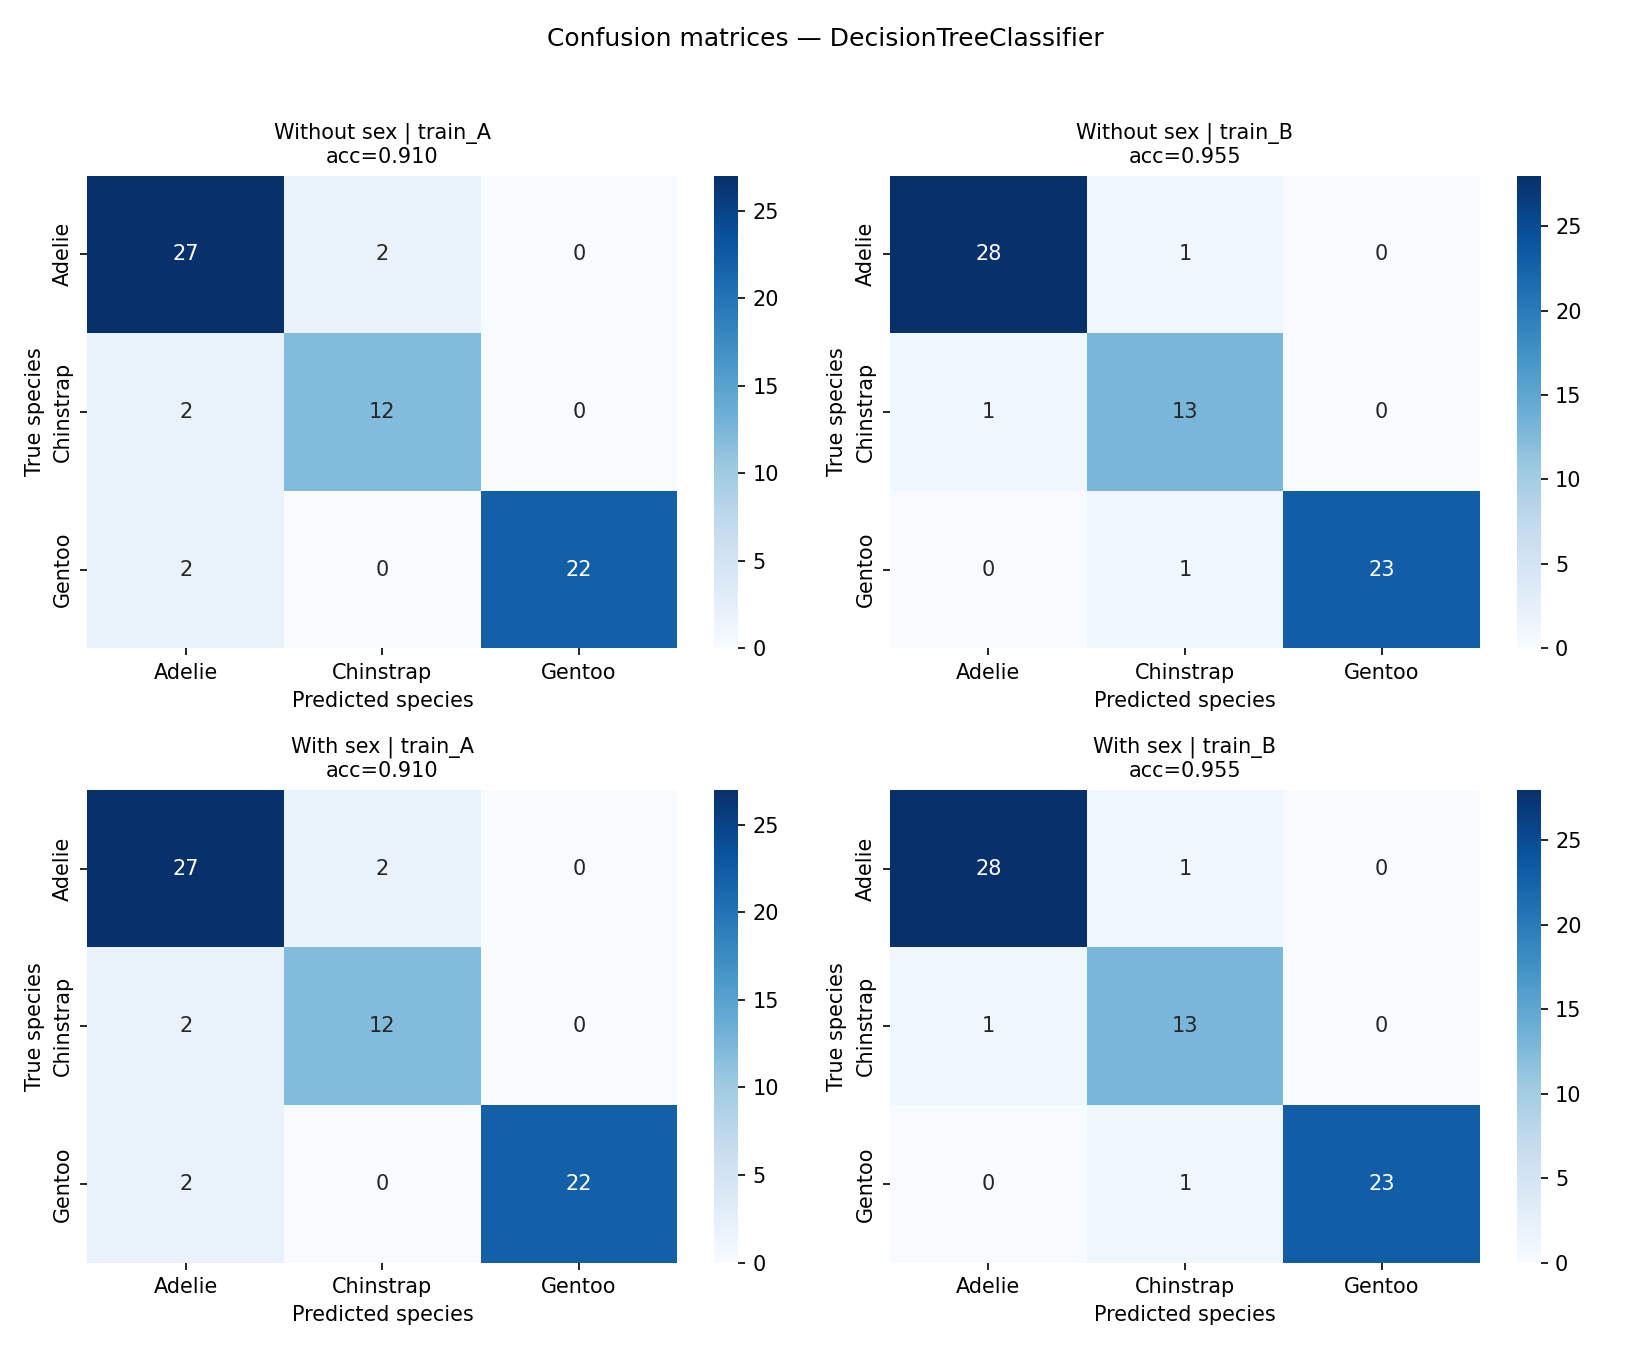
\includegraphics[width=0.95\textwidth]{figures/grid_DecisionTreeClassifier.png}
	\caption{Confusion matrices for the decision tree across feature configurations and training subsets.}
	\label{fig:grid_tree}
\end{figure}

\subsection{Stability in Regression}

Table~\ref{tab:reg_stability} reports R\textsuperscript{2} for each regressor on the shared test set, for the same four combinations.

\begin{table}[htbp]
	\centering
	\caption{Regression R\textsuperscript{2} across training subsets. The delta column is the change in R\textsuperscript{2} when sex is added.}
	\label{tab:reg_stability}
	\begin{tabular}{llccc}
		\toprule
		Model & Subset & Without sex & With sex & Delta \\
		\midrule
		Linear regression & train\_A & 0.712 & 0.770 & +0.058 \\
		Linear regression & train\_B & 0.711 & 0.786 & +0.075 \\
		Random forest     & train\_A & 0.756 & 0.806 & +0.050 \\
		Random forest     & train\_B & 0.793 & 0.841 & +0.048 \\
		\bottomrule
	\end{tabular}
\end{table}

For both regressors the delta is positive in both subsets, with ranges of 0.058 to 0.075 for linear regression and 0.048 to 0.050 for the random forest. The sign is consistent in all four runs, and the magnitude is also consistent for the random forest, which is a stronger signal than in classification. This matches the biological expectation: males and females differ systematically in body mass, and the sex variable provides information that the physical traits cannot fully recover on their own.

\subsection{Summary}

The A/B design isolates the effect of the training sample from the effect of the predictors. Across both studies, the sign of the effect of adding sex is the same in both training subsets, which supports the conclusion that the observed gains are real and not an artifact of a particular random split. The magnitude varies slightly between subsets, most likely because the test set is small, but the direction does not. The decision tree is the only case where sex has no measurable effect, and that is consistent with its ability to recover size-related splits directly from the physical traits.